\documentclass[a4paper,11pt, twocolumn]{article}
\usepackage[german, english]{babel} % Languages
\usepackage{tikz} % Tikz figures
\usepackage{siunitx} % SI-units package
\usepackage{bm} % Bold mathematics
\usepackage{listings} % Make listings, e.g. for code
\usepackage{enumitem} % Enumerate and itemize commands
\usepackage{multicol} % Make multiple columns for content
\usepackage[left=15mm, right=15mm, bottom=15mm, top=15mm, includeheadfoot]{geometry} % Modify geometry of page format
\usepackage{placeins} % For float barrier command
\usepackage{amsmath} % Math environments
\usepackage{fancyhdr} % Include the fancyhdr package
\usepackage{amsthm} % Theorem environments
\usepackage{siunitx} % Use SI
\usepackage{array} % Use array package for tables
\usepackage{tabularx} % Package to make nice tables
\usepackage{amssymb} % Math symbols
\usepackage{lipsum} % Provide dummy text
\usepackage{abstract} % Abstract package
\usepackage{nicefrac} % Nice fractions in in-line texts
\usepackage[hidelinks]{hyperref} % Make document with hyperlinks
\usepackage{cleveref} % Make references
\usepackage{subcaption} % Make subfigures
\usepackage{graphicx} % Make figures
\usepackage{mhchem} % Chemical notation
\usepackage{mathtools} % Various math tools
\usepackage{framed} % Frame equations
% Figure caption setup
\captionsetup{font=footnotesize,labelfont=bf}

% Python code listings
\definecolor{codegreen}{rgb}{0,0.6,0}
\definecolor{codegray}{rgb}{0.5,0.5,0.5}
\definecolor{codepurple}{rgb}{0.58,0,0.82}
\definecolor{backcolour}{rgb}{0.95,0.95,0.92}

\lstdefinestyle{mystyle}{
	backgroundcolor=\color{backcolour},   
	commentstyle=\color{codegreen},
	keywordstyle=\color{magenta},
	numberstyle=\tiny\color{codegray},
	stringstyle=\color{codepurple},
	basicstyle=\ttfamily\footnotesize,
	breakatwhitespace=false,         
	breaklines=true,                 
	captionpos=b,                    
	keepspaces=true,                 
	numbers=left,                    
	numbersep=5pt,                  
	showspaces=false,                
	showstringspaces=false,
	showtabs=false,                  
	tabsize=2
}

% Enumerate style
\renewcommand{\theenumi}{(\arabic{enumi})}
\renewcommand\labelenumi{\theenumi} % Change enumerate style from 1. to (1) etc.
\renewcommand{\theenumiii}{(\arabic{enumiii})}
\renewcommand\labelenumiii{\theenumiii} % Change enumerate style from 1. to (1) etc.
\setlist{itemsep = 0.2pt}

% Matrix and vector notation
\newcommand\matr[1]{\ensuremath{\boldsymbol{\mathbf{#1}}}}
\newcommand\vect[1]{\ensuremath{\bm{#1}}}
\newcommand\dint{\ensuremath{\int\displaylimits}}

% Units definitions
\DeclareSIUnit \parsec {pc}
\DeclareSIUnit \magnitudes {mag}

% Theorem environment
\newtheorem{tm}{Theorem}
\numberwithin{tm}{subsection}

% New tag form
\newtagform{normalsize}[\normalsize]{\normalsize(}{\normalsize)}

% Configure head- and footlines
\pagestyle{fancy} % Set head- and footlines
\fancyhead[C]{Adult face predicting machine} % Left headline
\fancyhead[L]{\nouppercase{\leftmark}} % Right headline
\fancyhead[R]{D. Zahnd, R. Zahnd}

\author{Daniel Zahnd}
\date{May 14, 2024 - \today}
\title{Building a homemade barometer \\ \vspace{0.5cm} \normalsize Theory and test report on building a homemade barometer}

\begin{document}

%\newgeometry{left=40mm,right=40mm}
\maketitle
%\newpage
%\pagenumbering{roman}
%\tableofcontents
%\FloatBarrier
%\newpage
%\pagenumbering{arabic}
%\setcounter{page}{1}


\begin{abstract}
Barometers are devices, that measure air pressure. Usually, this is done in the field of meteorology to explore future weather predictions. Observing the atmospheric pressure evolution at some fixed point in space allows for a rough estimate of possible future weather, since a pressure drop usually is a precursor for bad, and a pressure rise an indication for good weather. This paper is concerned with development of theory coupled with a simple realization and test of a homemade barometer.
\end{abstract}

\section{Introduction}
Barometers are used to measure air pressure. Observing the atmospheric pressure at a fixed point in space over a given time interval allows for coarse predictions of the future weather. This is due to the observation that pressure drops are usually linked to bad weather, while pressure rises often indicate development of good weather. 

High pressure air is heavier than low pressure air and thus has a tendency to sink due to buoyancy. Sinking air rises in temperature due to adiabatic and diabatic warming. Warm air can take up more water vapour and hence the relative humidity sinks. As a result, clouds tend to vanish and thus render precipitation unlikely. Low pressure air however tends to rise and thus to cool off with increasing height. Now, cold air is sooner saturated with water vapour than warm air. If air rises and cools off therefore, the air gets oversaturated with water vapour and hence clouds begin to form and precipitation becomes possible as well as likely.

As a rough estimate of the future weather helps with planning outdoor activities, it is nice to have a barometer at home to observe the pressure evolution. This paper hence aims to provide the necessary theory to build a homemade barometer using only equipment available in any hardware store. The general design of such a barometer will be provided here, whereas the details of an actual realization are left to the reader to figure out given the available tools and hardware.


\section{Theoretical foundation}
\subsection{Background}
The theoretical foundation of the proposed homemade barometer is comprised of two main equations and their theoretical background. 

The first equation is the ideal gas law \begin{equation}
	PV = Nk_B T,
\end{equation} where $P$ is the pressure of a gas, $N$ the number of particles in the volume $V$, $k_B$ the Boltzmann constant and $T$ the temperature of the gas. There are number of assumptions processed in the derivation of this ideal gas law; but for the purpose at hand it suffices to state that air pressure in non-extreme environments on earth follows the ideal gas law very well.

The second main equation is the equation of hydrostatic pressure \begin{equation}
	P = \rho g h,
\end{equation} where $P$ is the hydrostatic pressure of an incompressible fluid, $\rho$ is the density of the fluid, $g$ is the gravitational acceleration and $h$ is the depth in the fluid, where the hydrostatic pressure $P$ is measured.

\subsection{Working principle}
Consider an experimental setup as seen in \cref{fig:barometer_principle}. The experimental setup consists of a U-shaped tube with the opening facing towards the sky. At the bottom of the U, a valve is placed which separates both the left part and right part of the U. The right part of the U is furthermore closable, whereas the left part remains open throughout the experiment and is therefore subject to the atmospheric pressure $P_0$, which is to be measured. 

Initially, the red valve is closed and water is filled into the right and left part of the U. In the left end, the water is filled up to height $z_{l,0}$, whereas the water in the left tube is filled up to height $z_{r,0}$, fulfilling the condition $z_{r,0} \gg z_{l,0}$. After filling both ends of the U with water of density $\rho$, the right part of the U is closed, which means that at closed valve the pressure and volume of the residual air in the tube remains constant at $P_0$ and $V_0$. This situation is depicted in the left panel of \cref{fig:barometer_principle} and describes the experiment preparation required to carry out measurements.
\begin{figure}[h]
	\centering
	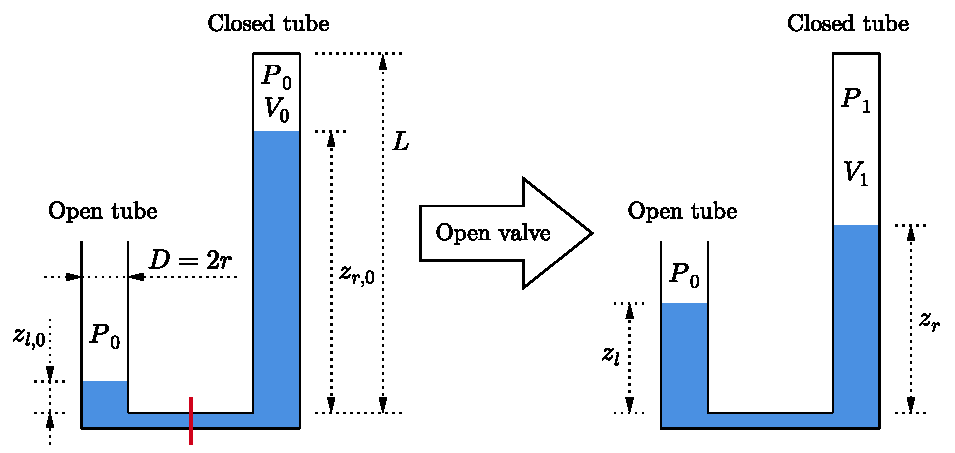
\includegraphics[width=0.5\textwidth]{figures/barometer_principle.pdf}
	\caption{General working principle of the proposed homemade barometer.}
	\label{fig:barometer_principle}
\end{figure}

Now, a measurement is carried out by first tediously preparing the experiment as described above. Then, the red valve is opened, which marks the starting point of the measurement process. Now, the water in the right part of the U is drawn to the left part of the U due to the higher hydrostatic pressure in the right part of the U. Water keeps flowing from the left part of the U to the right part until the sum of hydrostatic and atmospheric pressure in the right part of the U is exactly balanced by the sum of hydrostatic pressure and air pressure in the right (closed) part of the U. The water level in the left part of the U is now at $z_l$ and $z_r$ denotes the water level in the right part at equilibrium.

Mathematically speaking, the total pressure $P_l$ at the bottom of the U in the left part is given by \begin{equation}
	P_l = P_0 + \rho g z_l,
\end{equation} where analogously the total pressure $P_r$ at the bottom of the U in the right part is accounted for by \begin{equation}
P_r = P_1 + \rho g z_r.
\end{equation}
Now, at equilibrium, these two pressures must be equal to one another. Now, the pressure $P_1$ can further be expressed by means of the ideal gas law. Consider for this purpose the evolution of the residual air parcel located in the right part of the U. Initially, this air parcel exhibits pressure $P_0$ and a volume $V_0$. At equilibrium then, the pressure has dropped to $P_1$ due to an expanded volume $V_1 > V_0$. Considering the ideal gas law, the number of particles in the air parcel does not change from the initial condition to equilibrium, hence $N_0 = N_1 \doteq N$. Furthermore, the assumption $T_0 = T_1 \doteq T$ shall be made which means, that the temperature of the air parcel is assumed to stay constant throughout the measurement procedure. Writing out the ideal gas law for both initial and equilibrium conditions, one obtains \begin{equation}
	P_0V_0 = Nk_BT = P_1V_1 \quad \Leftrightarrow \quad P_1 = P_0\frac{V_0}{V_1}.
\end{equation} The volume $V_1$ can be expressed by means of the equation \begin{align}\begin{aligned}
V_1 &= V_0 + r^2\pi(z_{r,0}-z_r) \\ &= r^2\pi(L-z_{r,0})+r^2\pi(z_{r,0}-z_r) \\
&= r^2\pi (L-z_r).
\end{aligned}\end{align} The pressure $P_1$ can thus be expressed as \begin{equation}
P_1 = P_0 \frac{L-z_{r,0}}{L-z_{r}},
\end{equation} which renders the pressure $P_r$ at the bottom of the right U-part at equilibrum as \begin{equation}
P_r = P_0 \frac{L-z_{r,0}}{L-z_{r}} + \rho gz_r.
\end{equation} From the equilibrium condition $P_l \overset{!}{=} P_r$, the reasoning \begin{gather}
\begin{gathered}
	\overbrace{P_0 + \rho g z_l}^{P_l} = \overbrace{P_0 \frac{L-z_{r,0}}{L-z_{r}} + \rho gz_r}^{P_r} \\
	\Leftrightarrow \\
	P_0\left(1 - \frac{L-z_{r,0}}{L-z_{r}}\right) = \rho g(z_r - z_l)
\end{gathered}
\end{gather} Thus, the final barometer expression $P_0(z_{r,0}, z_r, z_l, L)$ results as a function of initial water height $z_{r,0}$, equilibrium water heights $z_r$ and $z_l$ in both parts of the U and the total length $L$ of the right U-part. This final equation is given by \begin{equation}\label{eq:barometer_equation}
P_0(z_{r,0}, z_r, z_l, L) = \rho g(z_r-z_l)\left(1-\frac{L-z_{r,0}}{L-z_{r}}\right)^{-1}.
\end{equation}
In \cref{fig:colormap_theory}, a visualization of the barometer equation \cref{eq:barometer_equation} for the parameters $L = \SI{1.99}{\meter}$, $z_{r,0} = \SI{1.16}{\meter}$, $g = \SI{9.81}{\meter\per\second\squared}$ and $\rho = \SI{1000}{\kilogram\per\cubic\meter}$ can be seen.
\begin{figure}[h]
	\centering
	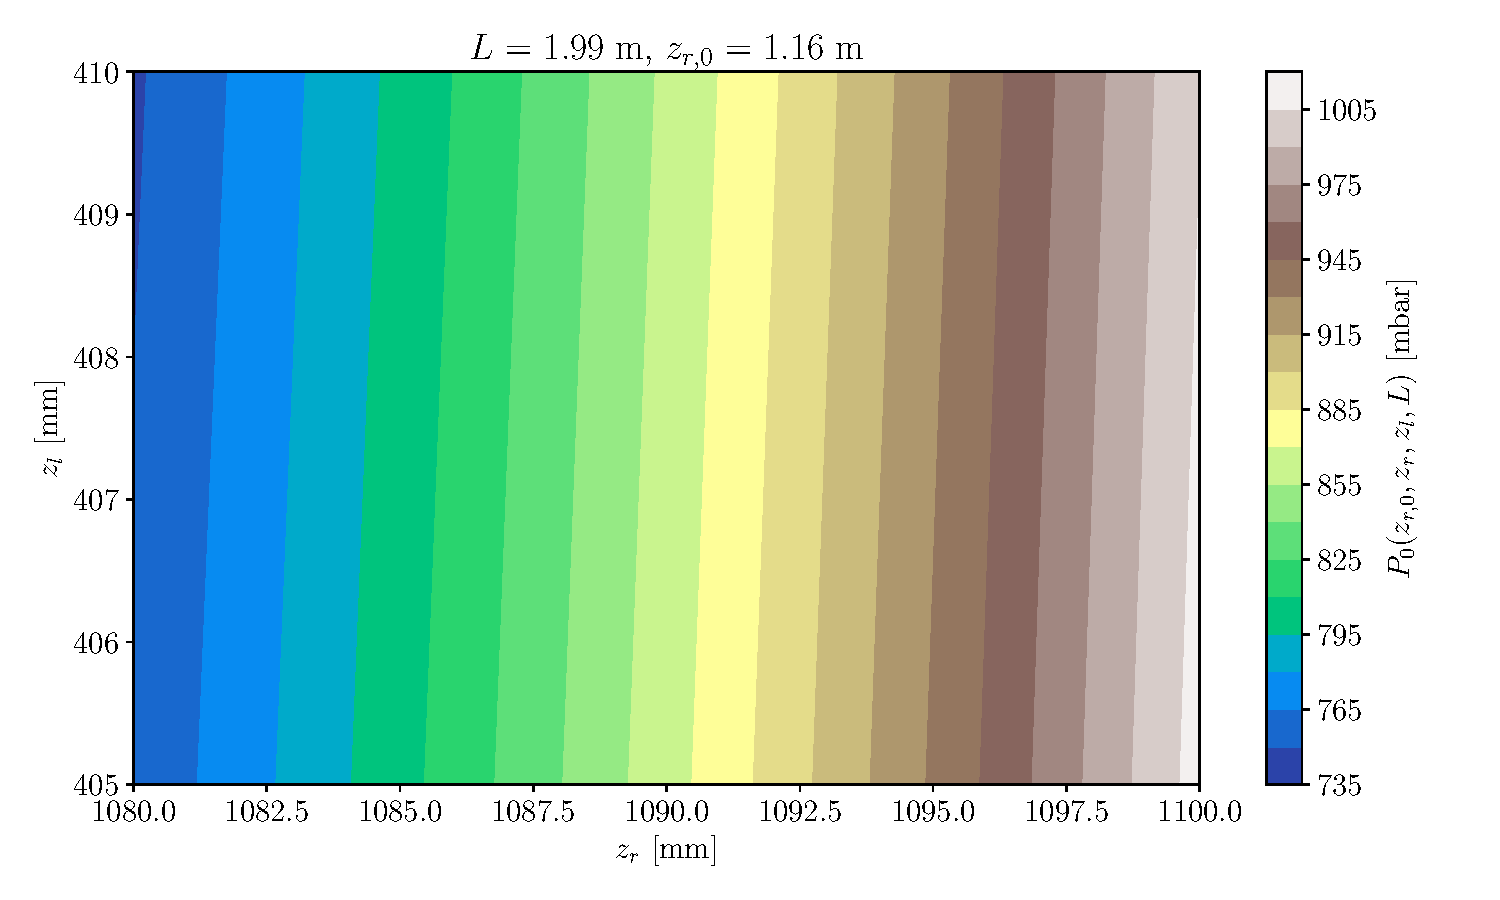
\includegraphics[width=0.5\textwidth]{figures/colormap_theory.pdf}
	\caption{Visualization of the barometer equation \cref{eq:barometer_equation}.}
	\label{fig:colormap_theory}
\end{figure}
As one can see from this figure, the difference $\Delta z \doteq z_{r,0}-z_r$ in water level height between initial and equilibrium conditions in the right part of the U increases with dropping ambient pressure $P_0$. This is not surprising insofar as with less ambient pressure $P_0$, the pressure exerted on the left water level is lower and hence the water level in the left part of the U will rise stronger as with less pressure. As a result, the water level in the right part of the U will drop lower at lower pressure, which makes the difference $\Delta z$ large.

The pressure regime in a practical experiment will range somewhere between $\SI{750}{\milli\bar}$ and $\SI{1000}{\milli\bar}$. Hence, following \cref{fig:barometer_principle} and \cref{fig:colormap_theory}, the barometer design will feature a tube length of $L \approx \SI{2.0}{\meter}$, an initial right water level of $z_{r,0} \approx \SI{1.1}{\meter}$ and an initial water height in the left part of the U of $z_{l,0} = \SI{33}{\milli\meter}$. This setup should result in a difference $\Delta z$ in the range of $\SI{60}{\milli\meter}$ to $\SI{90}{\milli\meter}$ between equilibrium and initial water level height in the right part of the barometric U.

\section{Methods}
\subsection{Experimental apparatus}
A homemade barometer was built according to the general sketch given in \cref{fig:barometer_principle}. The barometric U was made from transparent plastic tubing of inner diameter $D = \SI{10}{\milli\meter}$, which was attached to a wooden board of around 2 meters length using commercially available standard pipe clamps. At the bottom of the U, the valve was placed. Furthermore, a conic silicon plug of appropriate diameter was used to seal the right part of the barometric U airtight prior to measurements. The used materials are summarized in \cref{tab:materials} and were bought at the online shop temu.com\footnote{See \url{https://www.temu.com/}.}.

\begin{table}
\small
\centering
\begin{tabular}{|m{2.2cm}|m{2.2cm}|m{2.2cm}|}
	\hline
	\textbf{Description} & \textbf{Image} & \textbf{Link} \\
	\hline\hline
	Tube & \vspace{0.05cm}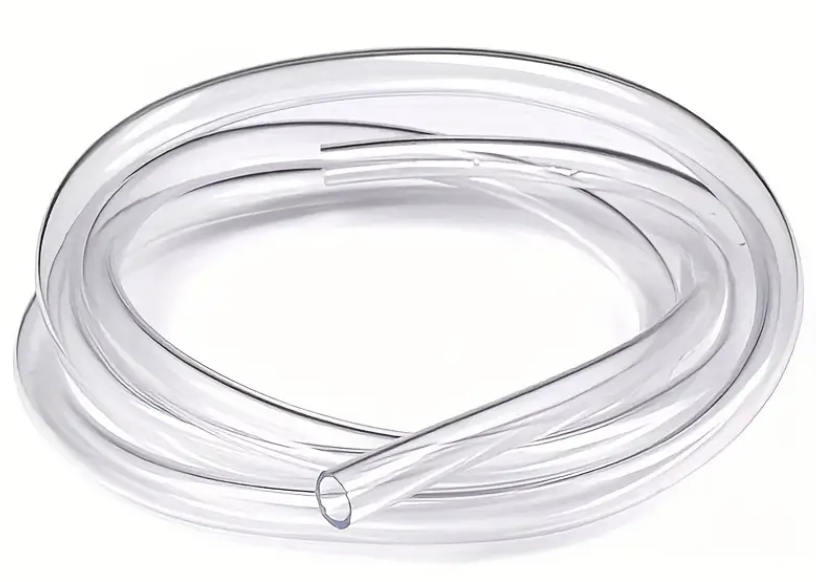
\includegraphics[width=2.0cm]{figures/tube.png}\vspace{0.05cm} & \href{https://www.temu.com/goods.html?_bg_fs=1&goods_id=601099518731564&sku_id=17592225551569&_x_msgid=192-20240730-05-B-760248003177005056-427-mMaeJZZR&_x_src=mail&refer_page_name=bgt_order_detail&refer_page_id=10045_1724253739572_on4iony7bd&refer_page_sn=10045&_x_sessn_id=ahq8utniw7}{tube-link} \\
	\hline
	Valve & \vspace{0.05cm}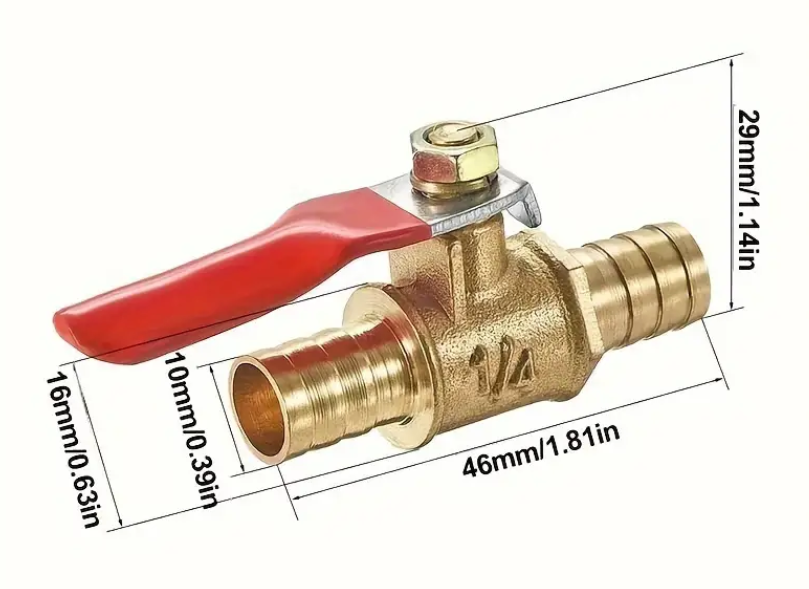
\includegraphics[width=2.0cm]{figures/valve.png}\vspace{0.05cm} & \href{https://www.temu.com/goods.html?_bg_fs=1&goods_id=601099549050111&sku_id=17592354223433&_x_msgid=192-20240730-05-B-760248003177005056-427-mMaeJZZR&_x_src=mail&refer_page_name=bgt_order_detail&refer_page_id=10045_1724253726270_l0vjc8ns90&refer_page_sn=10045&_x_sessn_id=ahq8utniw7}{valve-link} \\
	\hline
	Plug & \vspace{0.05cm}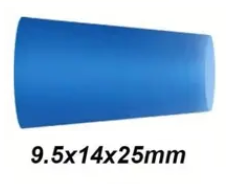
\includegraphics[width=2.0cm]{figures/plug.png}\vspace{0.05cm} & \href{https://www.temu.com/ch/100-teiliges-silikon-tapered-plug-set-7-grossen-1-16-bis-1-2-fur-lochversiegelung-pulverbeschichtung-lackierung-g-601099575024267.html?_oak_mp_inf=EIu1k7Wm1ogBGh1nb29kc19qb3Z1NGtfc29sZF9vdXRfc2ltaWxhciCo76eslzI%3D&top_gallery_url=https%3A%2F%2Fimg.kwcdn.com%2Fproduct%2Ffancyalgo%2Ftoaster-api%2Ftoaster-processor-image-cm2in%2F1cfc421a-0cec-11ef-88da-0a580a698089.jpg&spec_gallery_id=4145208100&refer_page_sn=10032&refer_source=10016&freesia_scene=25&_oak_freesia_scene=25&_oak_rec_ext_1=NTA5&_oak_gallery_order=1540174563%2C1937683670%2C1782981886%2C1294555810%2C2022719144&refer_page_el_sn=200970&_x_msgid=192-20240730-05-B-760248003177005056-427-mMaeJZZR&_x_src=mail&_x_sessn_id=ahq8utniw7&refer_page_name=goods&refer_page_id=10032_1724253860488_oc44p61c1o}{plug-link} \\
	\hline
\end{tabular}
\caption{Used materials for the homemade barometer reported in the paper at hand.}
\label{tab:materials}
\end{table}


\subsection{Measurement procedure}
The measurement procedure consists of two stages. 
\begin{figure}[h!]
	\centering
	\begin{subfigure}{0.22\textwidth}
		\centering
		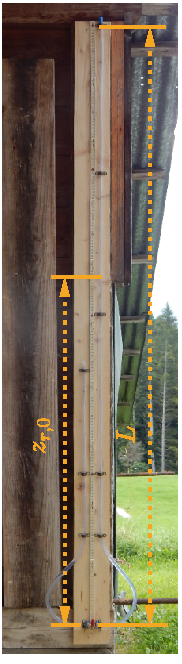
\includegraphics[width=\textwidth]{figures/initial.pdf}
		\caption{Barometer during stage 1 of a measurement.}
		\label{fig:meas_stage_1}
	\end{subfigure}
	\hfill
	\begin{subfigure}{0.22\textwidth}
		\centering
		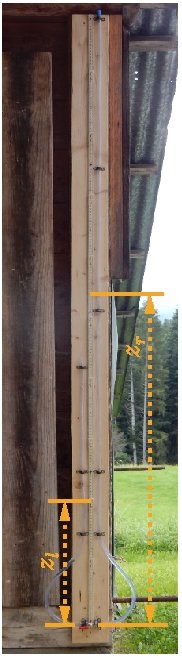
\includegraphics[width=\textwidth]{figures/final.pdf}
		\caption{Barometer during stage 2 of a measurement.}
		\label{fig:meas_stage_2}
	\end{subfigure}
	\caption{Pictures of the homemade barometer during both stages of a measurement procedure. At the top of the images, the blue plug used to seal the right part of the barometric U airtight, whereas on the bottom of the pictures, the red valve with the red lever can be perceived. In the left picture, the valve is closed, whereas in the right picture it is visualized in its open position.}
	\label{fig:measurement_procedure}
\end{figure}

In the first stage visualized in \cref{fig:meas_stage_1}, the valve is closed and water is filled into both arms of the barometric U, ensuring that $z_{l,0} \ll z_{r,0}$, such that the difference in hydrostatic pressure between both barometer arms is sufficient to be balanced by the difference in air pressure in stage 2 of the measurement. After the water has been filled into the barometric U, the top of the right part of the U is sealed by the blue plug. At this point, three measurements each for both $L$ and $z_{r,0}$ are taken.

In the second stage of a measurement, the valve is opened, which leads to an equilibration of hydrostatic and gas pressure in both barometric arms. A sufficient equilibrium is achieved as soon as the water levels are no more observed to oscillate in height. As soon as this condition has been reached, three measurements each for both $z_r$ and $z_l$ are acquired.

The successful completion of both stages will lead to 12 measurement values in total, three measurements per measured parameter $L$, $z_{r,0}$, $z_r$ and $z_l$. These values are then propagated through an uncertainty evaluation leading to a final value $P_0 \pm \sigma_{P_0}$ associated with an uncertainty $\sigma_{P_0}$ of measurement. The uncertainty $\sigma_{P_0}$ is given for a 95 percent confidence interval. 

All measurements were taken at Chrütli 128D, 3154 Rüschegg Heubach BE, which is situated at 1018 meters above sea level and coordinates \ang{46.762413} north and \ang{7.421758} east.

\subsection{Experiment 1: Plausibility test}
As a first experiment, a single measurement for the ambient pressure $P_0$ was conducted. This was done to test, if the homemade barometer gives plausible results within a reasonable uncertainty regime. The plausibility of the obtained results was compared to the values provided at the same time of measurement by an official weather station at a comparable height and not far away from the location of the homemade barometer; the chosen official weather station\footnote{See \href{https://www.meteoschweiz.admin.ch/service-und-publikationen/applikationen/messwerte-und-messnetze.html}{https://www.meteoschweiz.ch/messwerte} for measurement data obtained by this weather station.} is that of MeteoSchweiz in Plaffeien FR situated at 1044 meters above sea level and coordinates \ang{46.747717} north and \ang{7.266264} east.

\subsection{Experiment 2: Aiming for a weather prediction}
As a second experiment it was aimed for a prediction of a known weather trend. For this purpose, the ambient pressure $P_0$ was measured on two days approximately 24 hours apart. The first date and time of measurement was August 23, 2024 around 21:30, whereas the second date and time of measurement was August 24, 2024 around 21:00. For both of these measurements, the ambient pressure was measured three times. The observed dataset thus then consisted of six individual values, for which a trend can be visible.

August 23 was known to feature fair weather, whereas a change in weather to rainy condition on August 24 was predicted. If the measurements of ambient pressure obtained by the homemade barometer were to indicate this change of weather, a pressure drop from August 23 to August 24 would be expected.

\subsection{Uncertainty evaluation}
The measurement uncertainty for the experiment at hand is evaluated according to the standard procedure explained in \cite{GUM2023}.

\section{Results}

\subsection{Experiment 1: Plausibility test}
The photos depicted in \cref{fig:measurement_procedure} the plausibility experiment conducted on August 21, 2024 at 16:22 in the afternoon. The obtained values for the four measured parameters $z_{r,0}$, $z_r$, $z_l$ and $L$ are tabularized in \cref{tab:meas_values}.
\begin{table}[h]
	\small
	\centering
	\begin{tabular}{|c|c|c|c|}
		\hline
		\textbf{$z_{r,0}$ [mm]} & \textbf{$z_r$ [mm]} & \textbf{$z_l$ [mm]} & \textbf{$L$ [mm]} \\
	\hline\hline
	1159.0 & 1092.0 & 406.0	& 1989.0 \\
	\hline
	1158.0 & 1091.0 & 407.0	& 1988.0 \\
	\hline
	1158.5 & 1091.5 & 408.0 & 1987.0 \\
	\hline
	\end{tabular}
	\label{tab:meas_values}
	\caption{Obtained measurements of the four parameters for the plausibility experiment.}
\end{table}

The final result for the atmospheric pressure obtained by the measured values \cref{tab:meas_values} in combination with \cref{eq:barometer_equation} and an appropriate uncertainty budget according to the standard procedure explained in \cite{GUM2023} is given by \begin{equation}
	P_0 = 898.50 \pm 60.04 \text{ mbar},
\end{equation} where the uncertainty is given for a 95 percent confidence interval. 

In addition to the standard procedure for uncertainty evaluation according to \cite{GUM2023}, a Monte Carlo propagation of uncertainties was done to verify and complement the standard procedure. The results again for a 95 percent confidence interval are shown in \cref{fig:result_mc}.
\begin{figure}[h]
	\centering
	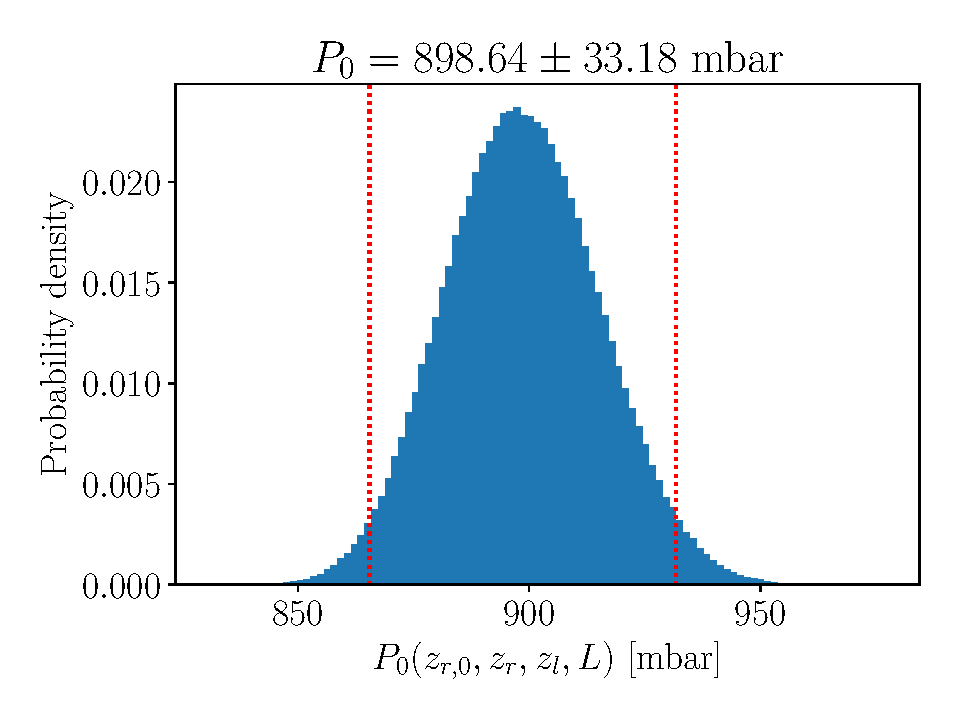
\includegraphics[width=0.35\textwidth]{figures/result_mc.pdf}
	\caption{Monte Carlo propagated uncertainties.}
	\label{fig:result_mc}
\end{figure}

As a reference value, the ambient pressure $P_{0,ref}$ measured at the MeteoSchweiz weather station located in Plaffeien at a similar height above sea level was taken to be \begin{equation}
	P_{0,ref} = 902.10 \text{ mbar}.
\end{equation}

\subsection{Experiment 2: Aiming for a weather prediction}
The obtained results for the ambient pressure $P_0$ for the mentioned two times of measurements are tabularized in \cref{tab:experiment_2_results}.
\begin{table}[h]
	\small
	\centering
	\begin{tabular}{|c|c|c|}
		\hline
		 \textbf{Date and time} & \textbf{$P_0$ [mbar]} & \textbf{$\sigma_{P_0}$ [mbar]} \\
		\hline\hline
		23.08.2024 21:31 &	840.74 &	53.25 \\
		\hline
		23.08.2024 21:34 &	824.49 &	50.75 \\
		\hline
		23.08.2024 21:37 &	834.59 &	55.64 \\
		\hline
		24.08.2024 20:56 &	830.72 &	49.72 \\
		\hline
		24.08.2024 20:59 &	803.48 &	52.02 \\
		\hline
		24.08.2024 21:02 &	809.41 &	53.34 \\
		\hline
	\end{tabular}
	\label{tab:experiment_2_results}
	\caption{Obtained results for the ambient pressure $P_0$ of experiment 2.}
\end{table} Furthermore, these values and their associated uncertainties are found graphed in \cref{fig:experiment_2_results} in order facilitate capturing a possible trend.
\begin{figure}[h]
	\centering
	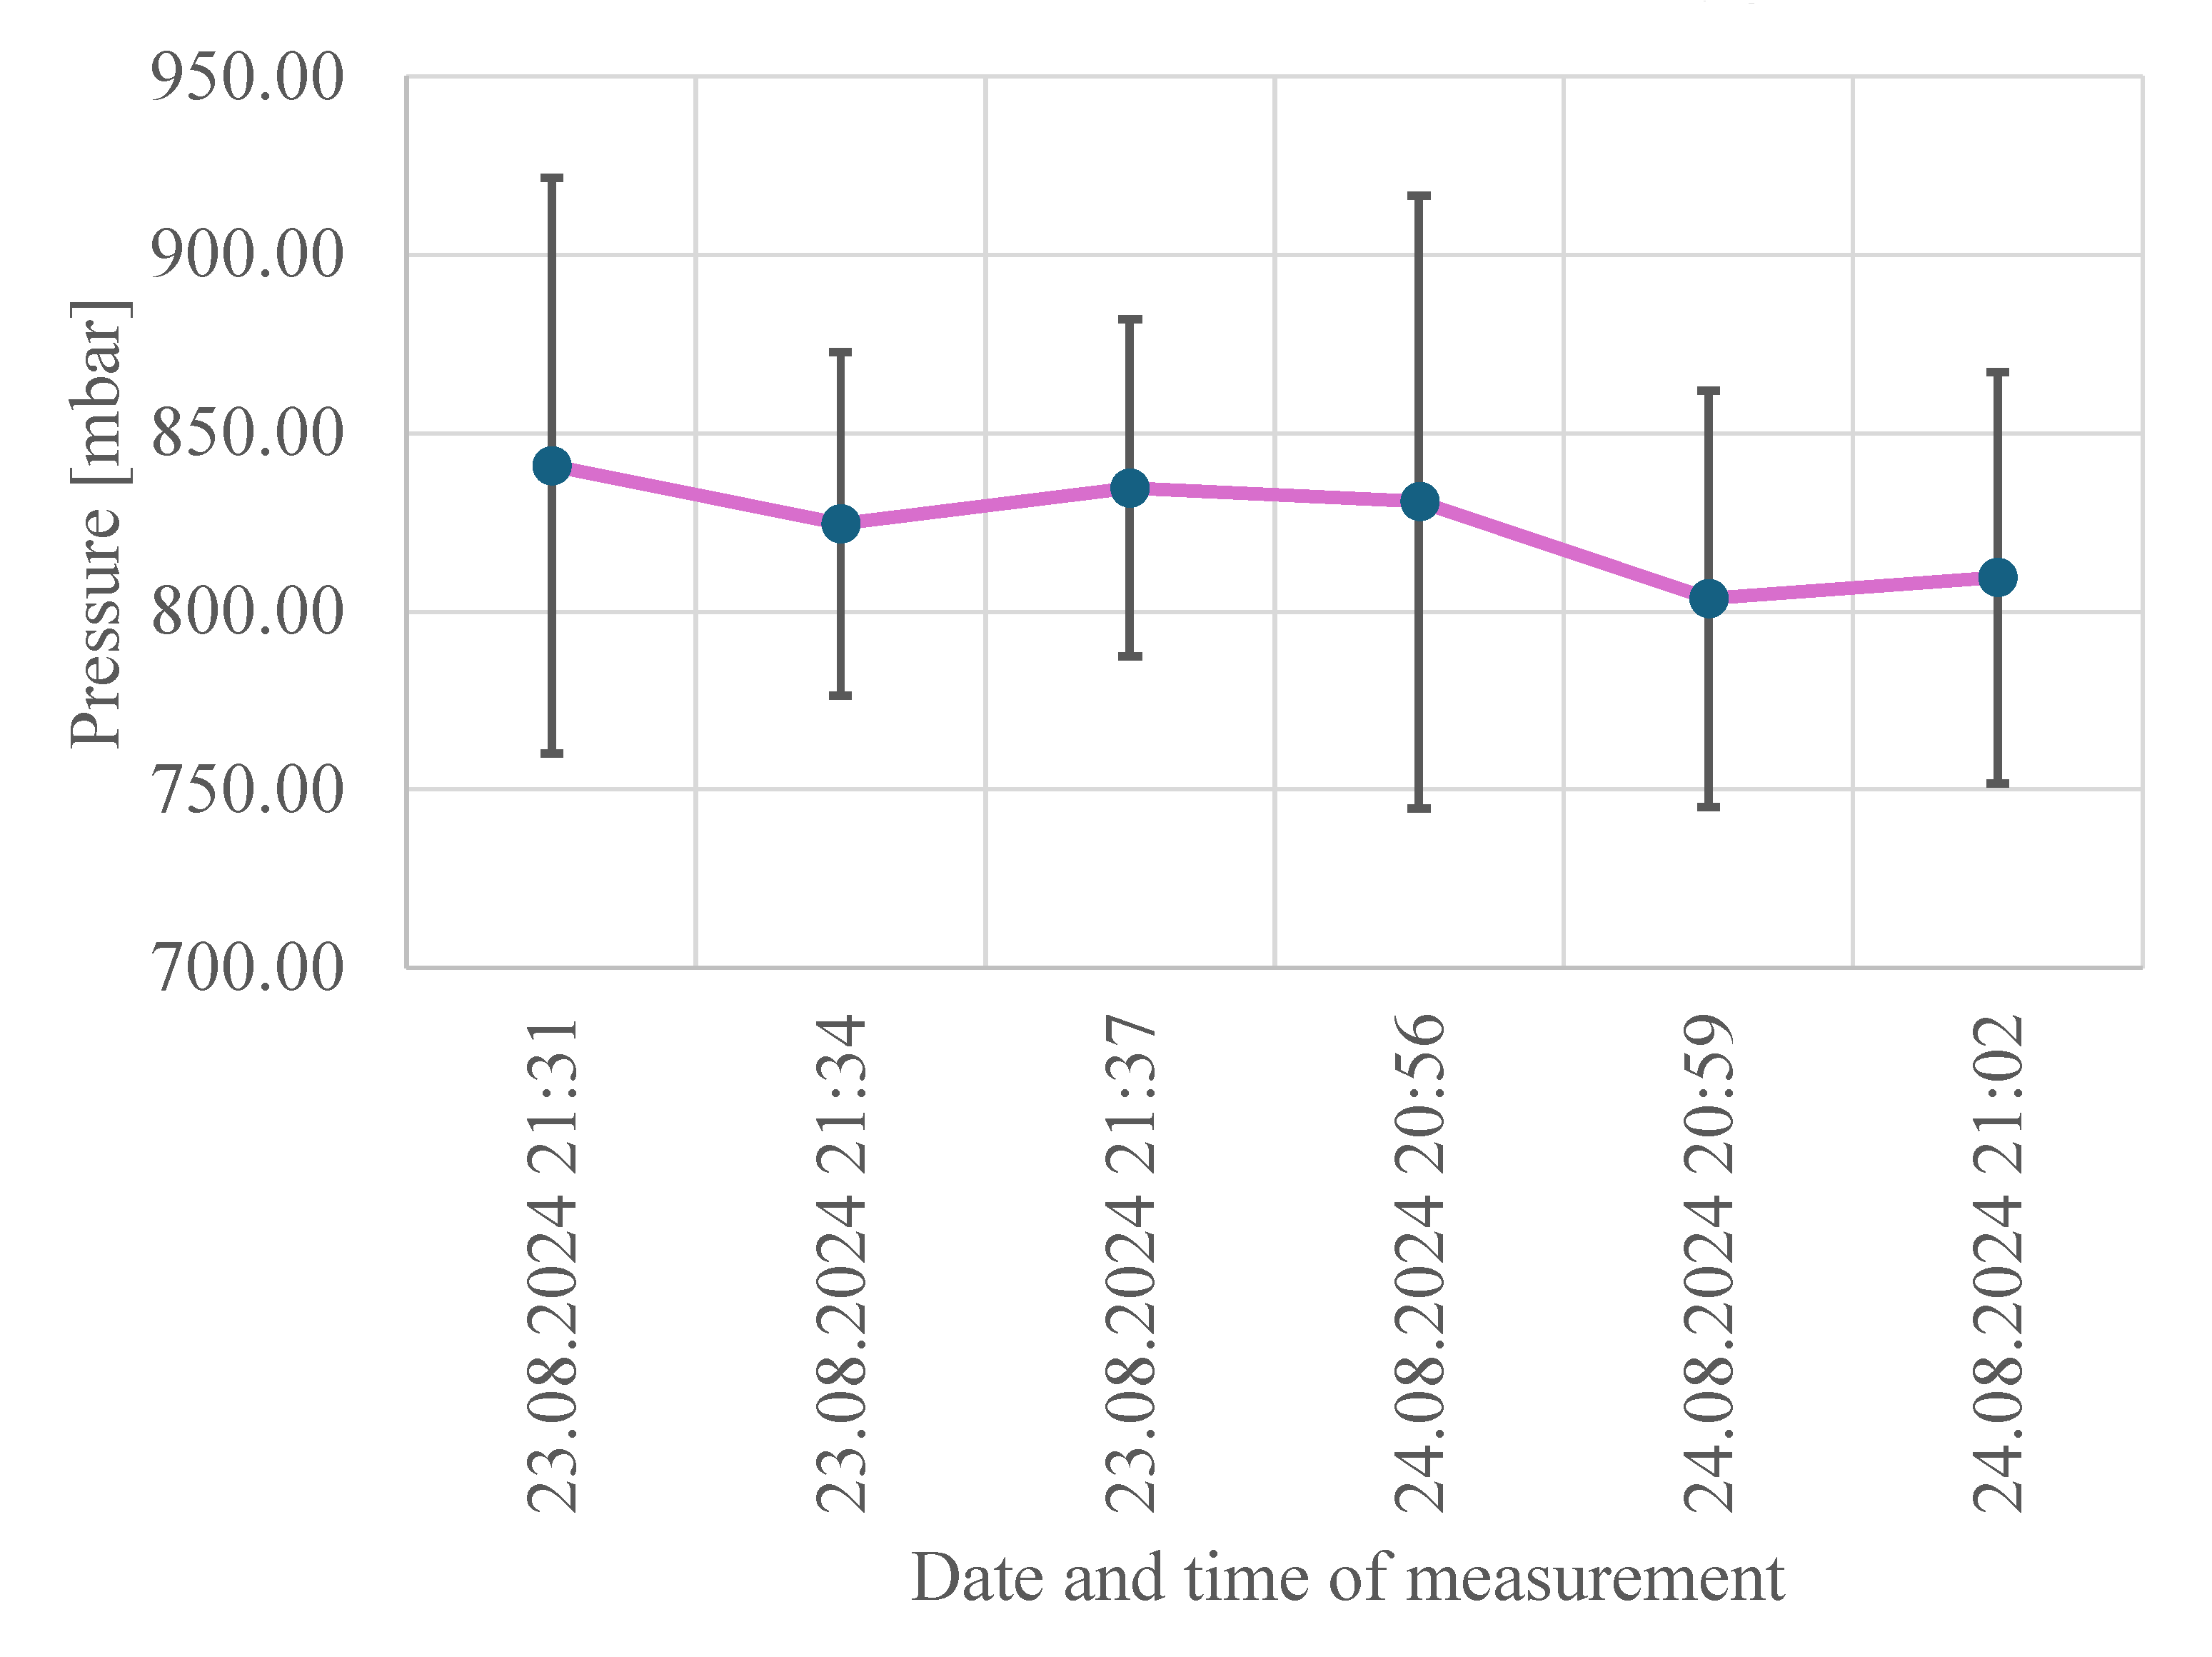
\includegraphics[width=0.4\textwidth]{figures/experiment_2_results_br.pdf}
	\caption{Graphed results as given in \cref{tab:experiment_2_results}.}
	\label{fig:experiment_2_results}
\end{figure} Details with respect to exact calculations and the uncertainty evaluation can be found below, aswell as in the code and spreadsheets available at the online repository\footnote{See \url{https://github.com/danielzahnd/various-documents/tree/main/homemade-barometer} for the complete material on the homemade barometer.}.

\subsection{Uncertainty evaluation}
There are four measured parameters, namely the total length $L$ of the right part of the barometric U, the initial right water height $z_{r,0}$, the final right water height $z_r$ and the final left water height $z_l$. Each of those measurements is in the units of length and measured by the same yard stick and thus subject to the same uncertainty contributions. However, some of the uncertainty contributions scale with measured length and are therefore different for each of the four parameters.

In the following material, each uncertainty contribution to each one of the four measured parameters is briefly described and explained. Details can be seen in the excel file used for the uncertainty evaluation available in the online repository\footnote{See \url{https://github.com/danielzahnd/various-documents/tree/main/homemade-barometer/code}.}. The total uncertainty reported is calculated by the formula \begin{equation}
	\sigma_{P_0} = 2\sqrt{U_{z_{r,0}}^2 + U_{z_r}^2 + U_{z_l}^2 + U_L^2},
\end{equation} with the involved quantities being explained below.

\paragraph{Initial right water height $z_{r,0}$} The initial right water height is subject to six considered uncertainty contributions. First of all, there is the statistical uncertainty contribution $\delta {z_{r,0}}$ given by the standard deviation of the three taken measurements. Second, there is an uncertainty contribution $\delta z_{r,0,rd}$ due to possibly incorrect reading of the yard stick. Third, there is an uncertainty associated to the surface tension of the water yielding a non-flat surface, given by $\delta z_{r,0,st}$. Fourth, a scaled uncertainty $\delta z_{r,0,mu}$ due to the accuracy class of the used yard stick contributes to the budged. Fifth, there is a contribution $\delta z_{r,0,or}$ due to a possible misidentification of the measurement origin down at the bottom of the barometric U. Sixth, there is a contribution $\delta z_{r,0,tilt}$ due to a possible tilt of the experimental apparatus, thus also scaling with measured length. 

The total uncertainty contribution $U_{z_{r,0}}$ of the initial right water height $z_{r,0}$ is thus given by \begin{equation}
	U_{z_{r,0}}^2 = \left(\frac{\partial P_0(z_{r,0}, z_r, z_l, L)}{\partial z_{r,0}}\right)^2\sum_{i}\delta z_{r,0,i}^2.
\end{equation}

\paragraph{Final right water height $z_r$} The final right water height $z_r$ is subject to the same, but appropriately scaled uncertainty contributions as $z_{r,0}$. Thus, there is the statistical contribution $\delta z_r$, the contribution $\delta z_{r,rd}$ due to reading, the quantity $\delta z_{r,st}$ due to surface tension, the contribution $\delta z_{r,mu}$ given by the accuracy class of the yard stick, the uncertainty $\delta z_{r,or}$ due to possible origin misplacement and finally the contribution $\delta z_{r,tilt}$ caused by possible tilt.

The total uncertainty contribution $U_{z_{r}}$ of the final right water height $z_{r}$ is thus given by \begin{equation}
	U_{z_{r}}^2 = \left(\frac{\partial P_0(z_{r,0}, z_r, z_l, L)}{\partial z_{r}}\right)^2\sum_{i}\delta z_{r,i}^2.
\end{equation}

\paragraph{Final left water height $z_l$} The final left water height $z_l$ is subject to the same, but appropriately scaled uncertainty contributions as $z_{r}$. Therefore, there is the statistical contribution $\delta z_l$, the contribution $\delta z_{l,rd}$ due to reading, the quantity $\delta z_{l,st}$ due to surface tension, the contribution $\delta z_{l,mu}$ given by the accuracy class of the yard stick, the uncertainty $\delta z_{l,or}$ due to possible origin misplacement and finally the contribution $\delta z_{l,tilt}$ caused by possible tilt.

The total uncertainty contribution $U_{z_{l}}$ of the final left water height $z_{l}$ is thus given by \begin{equation}
	U_{z_{l}}^2 = \left(\frac{\partial P_0(z_{r,0}, z_r, z_l, L)}{\partial z_{l}}\right)^2\sum_{i}\delta z_{l,i}^2.
\end{equation}

\paragraph{Tube length $L$} The tube length $L$ is subject to the same, but appropriately scaled uncertainty contributions as $z_{l}$, except for the surface tension contribution, since with $L$ no water level measurements are involved. Hence, there is the statistical contribution $\delta L$, the contribution $\delta L_{rd}$ due to reading, the uncertainty $\delta L_{mu}$ given by the accuracy class of the yard stick, the uncertainty $\delta L_{or}$ due to possible origin misplacement and finally the contribution $\delta L_{tilt}$ caused by possible tilt.

The total uncertainty contribution $U_{L}$ of the tube length $L$ is thus given by \begin{equation}
	U_{L}^2 = \left(\frac{\partial P_0(z_{r,0}, z_r, z_l, L)}{\partial L}\right)^2\sum_{i}\delta L_{i}^2.
\end{equation}

\section{Discussion}
Concerning the first experiment, one can state that the homemade barometer works pretty well, considering that the deviation to the reference value is only about 5 mbar. However, other measurements and corresponding reference values were taken and the seen deviations range from 5 to up about 100 mbar; hence, the measurement reported as a first experiment seems to be a ``lucky'' value, since the difference to the reference value is so low. However, the general pattern recorded by the reference weather station also seems to be reflected by the homemade barometer measurements; this is to say that pressure rises and falls do coincide for both the reference weather station measurements and those of the homemade barometer. It is to be remarked at this point, that the Monte Carlo simulation of uncertainty propagation leads to a smaller 95 percent confidence interval uncertainty than the standard procedure does. Further work could elaborate on finding the reason for this observation; likely, this is linked to the fact, that not all uncertainty contributions follow the same probability distributions.

As for the second experiment, is was observed that the measurements obtained by the homemade barometer tend to be around 70 mbar lower on average than those of the reference weather station. This indicates, that there is some systematic measurement error present in the experimental setup. It would be a future improvement to find and correct this systematic issue. Apart from that, the observed weather tendency seemed to correspond to the observed slight pressure drop; from the 23th to the 24th of August, the weather shifted from fair to rainy. Also, there was a pressure drop recorded, as can be seen from \cref{fig:experiment_2_results}. However, the uncertainty ranges are fairly large compared to the absolute values, the average relative measurement uncertainty for the measurements reported in \cref{tab:experiment_2_results} is around $7\cdot 10^{-2}$. This means the data seen in \cref{fig:experiment_2_results} permit to draw negative, but also slightly positive slope trend lines. Hence, no actual statement is possible from the obtained data and the associated uncertainties, if the data indeed do indicate a falling pressure or if this is not the case.

\section{Conclusions}
One can conclude from the reported material, that the homemade barometer indeed does work; however, it seems that the device is fairly inaccurate at present stage, such that it does not allow for reliable weather development presumptions. The reason behind this is that pressure fluctuations linked to changes in weather usually do not exceed 50 mbar; which is the current range of measurement uncertainty of the device. Hence, one could draw positive or negative slope trendlines through acquired data and therefore making reliable predictions for the weather development impossible.

It can however be stated, that the general principle of the homemade barometer indeed works. There are also possibilities for improvement; one could for example increase the length $L$ and the initial right water height $z_{r,0}$, such that the observed difference $\Delta z = z_{r,0}-z_r$ would be larger than at present stage and thus making the uncertainty contributions due to reading and other sources less significant. There are also many other possibilities to improve the device, for example making the seal of the right part of the barometric U more reliable; currently, a silicon plug is used for that purpose of which the author is unsure, whether it really seals the tube airtight or not. Exploring and implementing further improvements would be the task of future work concerning the reported homemade barometer.

Summing it up it can be said, that building a homemade barometer is a fun science project one can do with househeld tools at home, for example with kids or family. It would also make for a cool science project in middle or high schools.

\appendix
\section{Derivation of the ideal gas law}
The ideal gas law can be derived from the so-called kinetic gas theory. The kinetic gas theory is based on three postulates, which can be found in any physics textbook such as \cite{tipler2007physics}:
\begin{enumerate}
	\item The volume of the gas under consideration contains a large number of molecules.
	\item The adjacent molecules are separated at distances much larger than their sizes.
	\item The only interactions between molecules are elastical collisions.
\end{enumerate}
Given these three postulates, the so-called Maxwell-Boltzmann distribution for the absolute value $v$ of molecules in a gas can be derived; it is given by \begin{equation}
	p(v) = 4\pi v^2\left(\frac{m}{2\pi k_BT}\right)^{3/2}e^{-\frac{mv^2}{2k_B T}},
\end{equation} where $p(v)$ is the probability, that the velocity $v$ of a molecule in the gas is found to be in the interval $v \in [v, v + \mathrm{d}v ]$. Furthermore, $m$ denotes the mass of a gas molecule. Since $p(v)$ is a probaility density function, the mean squared velocity $\bar{v^2}$ of a gas molecule can be calculated by means of performing the integral \begin{equation}\label{eq:mean_squared_velocity}
\overline{{v^2}} = \int_{0}^{\infty}v^2 p(v)\,\mathrm{d}v = \frac{3k_B T }{m},
\end{equation} where $k_B$ is known as the Boltzmann constant.

Now, in order to derive an expression for the pressure $P$, one can consider a cubic box of length $l$ filled with $N \in \mathbb{N}$ gas molecules following the kinetic gas theory. Such a situation is visualized in \cref{fig:ideal-gas-law-derivation}.
\begin{figure}[h]
	\centering
	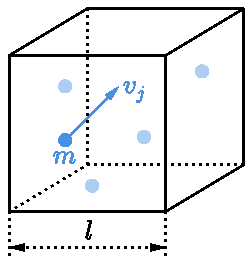
\includegraphics[width=0.15\textwidth]{figures/ideal-gas-law-derivation.pdf}
	\caption{Illustration of a gas container.}
	\label{fig:ideal-gas-law-derivation}
\end{figure} Each molecule $j \in \{1,\dots,N\}$ shall have a velocity $\vect{v}_j = (v_{j,x}, v_{j,y}, v_{j,z})^\top$ and a mass $m$. The pressure exerted on a container wall is hence given by the total force $F$ generated by molecules hitting the wall divided by the surface $A = l^2$ of the wall. The force $F$ exerted by molecules hitting a container wall is given by the change in momentum of the hitting particles divided by the interval of time, during which the change in momentum occurs; therefore, one can write down \begin{equation}
F = \sum_{j = 1}^{N}\frac{m v_{j,i}^2}{l} = \frac{1}{3}\sum_{j = 1}^{N}\frac{m v_{j}^2}{l},
\end{equation} where in the last step \begin{equation}
\sum_{j = 1}^{N}v_{j,x} = \sum_{j = 1}^{N}v_{j,y} = \sum_{j = 1}^{N}v_{j,z} = \frac{1}{3}\sum_{j = 1}^{N}v_j^2
\end{equation} with $v_j = |\vect{v}_j|$ was used, since no particular direction of movement is preferred by the gas molecules. Now, the pressure $P$ can be calculated by the force $F$ divided by the surface area $A = l^2$ as \begin{equation}
P = \frac{F}{A} = \frac{m}{3V}\sum_{j = 1}^{N} v_j^2.
\end{equation} The average kinetic energy $\frac{1}{2}m\overline{{v^2}}$ can be calculated by means of \begin{equation}
\frac{1}{2}m\overline{{v^2}} = \frac{1}{2N}\sum_{j=1}^{N} m v_j^2,
\end{equation} which allows for a reformulation of the former equation as \begin{equation}\label{eq:ideal_gas_law_almost_final}
PV = \frac{N}{3}m\overline{{v^2}} = \frac{2N}{3f}\bar{E}_f,
\end{equation} where $\bar{E}_f \doteq \frac{f}{2}m\overline{{v^2}} = f\bar{E}$ with $\bar{E} = \frac{1}{2}k_B T$ the average energy per degree of freedom $f$ of movement was defined. Thus, $\bar{E}_f$ is the average kinetic energy of a molecule with $f$ degrees of freedom of movement. In the case of single-atom molecules, the result \cref{eq:mean_squared_velocity} holds and one has \begin{equation}
\frac{1}{2}m\overline{{v^2}} = \frac{3}{2}k_B T = 3\bar{E}.
\end{equation} From this, $f=3$ can be concluded for single-atom molecules, which corresponds to the expected three degrees of translational freedom. Inserting the above expressions for $\bar{E}$ and $\bar{E}_f$ into \cref{eq:ideal_gas_law_almost_final} yields the ideal gas law \begin{equation}
PV = Nk_B T.
\end{equation}

% Derive the ideal gas law from first principles clearly stating the assumptions flowing into the derivation.

\section{Derivation of hydrostatic pressure}
Hydrostatic pressure is the pressure an object experiences on its surface due to a medium of different density $\rho$ surrounding it, the whole system being subject to a gravitational field. Consider therefore for a derivation of the mathematical expression for the hydrostatic pressure \cref{fig:hydrostatic-pressure-derivation}.
\begin{figure}[h]
	\centering
	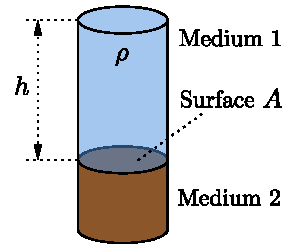
\includegraphics[width=0.15\textwidth]{figures/hydrostatic-pressure-derivation.pdf}
	\caption{Illustration of an object (medium 2) experiencing hydrostatic pressure exerted on it by an other medium (medium 1) of constant density $\rho$.}
	\label{fig:hydrostatic-pressure-derivation}
\end{figure}

The hydrostatic pressure $P$ exerted on medium 2 by means of medium 1 is given by the gravitational force generated by the mass of medium 1 divided by the surface area of medium 2 facing medium 1. Hence, one can write \begin{equation}
	P = \frac{\rho h A g}{A}  = \rho g h.
\end{equation}  % Derive hydrostatic pressure with a sketch.

%\section{Measurement uncertainty evaluation}
%\subsection{Random variable}
%A random variable is some quantity $x$, which can take a random value. Those random values follow a certain probability distribution, which is determined by the underlying process constituting the random variable.If the probability distribution of a random variable is known, the probability density $p(x)$ can be written down for the continuous and discrete cases as \begin{equation}
%	\int_{-\infty}^{\infty}p(x)\,\mathrm{d}x = 1 \qquad \text{and} \qquad \sum_{i} p(x_i) = 1.
%\end{equation}
%
%\subsection{Expectation value}
%The expectation value $E(x) \doteq \bar{x}$ of a random variable $x$ for both the continuous and discrete case is defined as \begin{equation}
%	E(x) = \int_{-\infty}^{\infty}xp(x)\,\mathrm{d}x
%	\end{equation}
%	and
%	\begin{equation}
%	E(x) = \sum_{i}x_ip(x_i).
%\end{equation}
%
%\subsection{Variance, standard deviation and covariance}
%The variance $V(x)$ of a continuous or discrete random variable $x$ can be calculated by means of \begin{equation}
%	V(x) = \int_{-\infty}^{\infty} (x-\bar{x})^2\,\mathrm{d}x \end{equation} and
%	
%	\begin{equation} V(x) = \sum_{i} (x_i-\bar{x})^2p(x_i).
%\end{equation}
%The standard deviation $\sigma_x$ is defined as the square root of the variance, hence \begin{equation}
%	\sigma_x = \sqrt{V(x)}.
%\end{equation}
%Let now $x_1,\dots,x_n$ be random variables with associated probability densities $p(x_j)$, $j\in \{1,\dots,n\}$ and joint probability densities $p(x_i,x_j)$. Let furthermore be $\bar{x}_i = E(x_i)$. The covariance $K(x_i,x_j)$ of two random variables for the continuous and discrete case is defined as \begin{gather}\label{eq:covariance}\footnotesize
% \begin{gathered}
%	K(x_i,x_j) = \int_{-\infty}^{\infty}\int_{-\infty}^{\infty}(x_i-\mu_i)(x_j-\mu_j)p(x_i,x_j)\,\mathrm{d}x_i\,\mathrm{d}x_j
%\end{gathered}\end{gather} and \begin{equation}
%	K(x_i,x_j) = \sum_{k,l}(x_{i_k}-\mu_{i})(x_{j_l}-\mu_j)p(x_{i_k},x_{j_l}).
%\end{equation} In the context of covariance, one usually also defines the correlation coefficient $\rho(x_i,x_j)$ between two random variables as \begin{equation}\label{eq:correlationcoefficient}
%	\rho(x_i,x_j) = \frac{K(x_i,x_j)}{\sqrt{V(x_i)V(x_j)}} = \frac{K(x_i,x_j)}{\sigma_{x_i}\sigma_{x_j}}.
%\end{equation} If one has two discrete random variables $a$ and $b$ following a uniform distribution and samples $\{a_1,\dots,a_n\}$ and $\{b_1,\dots,b_n\}$ with $n\in \mathbb{N}$, one can calculate an estimate $s(a,b)$ of the covariance $K(a,b)$ as \begin{equation}
%	s(a,b) = \frac{1}{n-1}\sum_{i=1}^{n} (a_i-\bar{a})(b_i-\bar{b}).
%\end{equation}
%
%\subsection{Propagation of uncertainties}
%Consider some random variables $x_1,\dots,x_n$ and a function $f(x_1,\dots,x_n)$ relating those variables. Let furthermore $\sigma_{x_i}$ be the uncertainties (standard deviations) of the random variables $x_i$ and let $\sigma_{x_ix_j} = \sqrt{K(x_i,x_j)}$ be the joint uncertainties of $x_i$ and $x_j$. In this case, the general propagation of uncertainties $\sigma_{x_i}$ on the outcome $f(x_1,\dots,x_n)$ is quantified by the uncertainty $\sigma_f$ as \begin{gather}\label{eq:generallawpropagationofuncertainties}
%\footnotesize	\begin{gathered}\sigma_f = \sqrt{\sum_{i=1}^{n}\left(\frac{\partial f}{\partial x_i}\right)^2 \sigma_{x_i}^2+ 2\sum_{1\leq i<j\leq n}\left(\frac{\partial f}{\partial x_i}\right)\left(\frac{\partial f}{\partial x_j}\right)\sigma_{x_ix_j}^2}.
%\end{gathered}\end{gather}

\section{Propagation of uncertainties}
The following formulae are derived in detail in standard references such as \cite{GUM2023}.

Consider $n \in \mathbb{N}$ random variables $x_1,\dots,x_n$ and a function $f(x_1,\dots,x_n)$ relating those variables. Let furthermore $\sigma_{x_i}$ be the uncertainties (standard deviations) of the random variables $x_i$, which are assumed to be uncorrelated. In this case, the general propagation of uncertainties $\sigma_{x_i}$ on the outcome $f(x_1,\dots,x_n)$ is quantified by the uncertainty $\sigma_f$ as \begin{gather}\label{eq:generallawpropagationofuncertainties}
		\begin{gathered}\sigma_f = \sqrt{\sum_{i=1}^{n}\left(\frac{\partial f}{\partial x_i}\right)^2 \sigma_{x_i}^2} = \sqrt{\sum_{i=1}^{n}c_i^2 \sigma_{i}^2},
\end{gathered}\end{gather} where the short-hand notation $\sigma_i \doteq \sigma_{x_i}$ and $c_i \doteq \partial f/\partial x_i$ was introduced. Note, that the $c_i$ factors are commonly called sensitivity coefficients.

% Include basics about calculating measurement uncertainty by Gauss' error propagation. Mention assumptions made (rectangular distr., normal distr. multiplicative factors) and result is normally distributed. See METAS documentation and PhD notes.

%\end{multicols}

\bibliography{references}
\bibliographystyle{apalike}

\end{document}